\documentclass[conference]{IEEEtran}

\usepackage{cite}
\usepackage{amsmath,amssymb,amsfonts}
\usepackage{algorithmic}
\usepackage{graphicx}
\usepackage{subfigure}
\usepackage{textcomp}
\usepackage{xcolor}
\usepackage{tabularx, booktabs}

\newcolumntype{L}{>{\centering\arraybackslash}m{2cm}}

\def\BibTeX{{\rm B\kern-.05em{\sc i\kern-.025em b}\kern-.08em
    T\kern-.1667em\lower.7ex\hbox{E}\kern-.125emX}}
\begin{document}

% --------- Title ----------- 
\title{Mining Patterns in Higher Education Enrollment Data}

% --------- Authors section -----------
\author{\IEEEauthorblockN{Ravi Bharadwaj C}
\IEEEauthorblockA{\textit{CS-IS department} \\
\textit{BITS Pilani, Hyderabad campus}\\
Hyderabad, India \\
f20160244@hyderabad.bits-pilani.ac.in}
\and
\IEEEauthorblockN{Shekhar Somani}
\IEEEauthorblockA{\textit{CS-IS department} \\
\textit{BITS Pilani, Hyderabad campus}\\
Hyderabad, India \\
f20160347@hyderabad.bits-pilani.ac.in}
\and
\IEEEauthorblockN{Maneesh Sistla}
\IEEEauthorblockA{\textit{CS-IS department} \\
\textit{BITS Pilani, Hyderabad campus}\\
Hyderabad, India \\
f20170238@hyderabad.bits-pilani.ac.in}
}

\maketitle

% --------- Abstract -----------
\begin{abstract}
The aim of this paper is to find patterns, relationships and draw insights from enrollment statistics of higher eduction in India. The data contains census of the population of each college, split by caste, gender and religion, and also contains details about the enrolled courses. This paper details the use of three techniques to identiy patterns in this dataset - Frequent pattern mining using Apriori rule, Clustering using K-means and Classification using logistic regression and a neural network approach. The paper details the complete process followed in completing the data mining tasks by describing the problem, the data selection, pre-processing, visualization, and the mining tasks. The resulting patterns and relationships are presented at the end of the paper comparing the results from each of the three mining techniques while also detailing the advantages and disadvantages of using the three techniques on this dataset which can be generalized to a high dimensional categorical data along with highly sparse ratio data (census).
\end{abstract}

\begin{IEEEkeywords}
Data mining, Apriori, K-means, classification, pre-processing
\end{IEEEkeywords}

% --------- 1. Introduction -----------
\section{Introduction}
This research project aims to analyze the student enrollment patterns in higher education programmes across India in the year of 2015. The aim is to analyze and find relationships and patterns between different factors that affect enrollment in a particular degree or college. The dataset is obtained from Indian government data website \cite{b1}. This dataset contains 400,000+ entries of programmes which show the types of students enrolled in different higher education programmes. 

Different pre-processing techniques are applied on the dataset to make the data more suitable for use in visualizations as well as data mining tasks. After visualizing the data, data mining tasks are performed on the dataset to obtain the desired relationships and patterns. Three data mining techniques are explored in this paper and are applied on this data set. The three techniques are as follows:
\begin{itemize}
    \item Association rule mining using the Apriori algorithm \cite{b2}
    \item Clustering using the K-means algorithm \cite{b3}
    \item Classification using logistic regression and a neural network
\end{itemize} 

All the pre-processing techniques, visualizations, and all the three data mining techniques were implemented in python3 with the help of jupyter notebooks and the complete implementation of this paper can be found on GitHub.

% --------- 2. Problem definition -----------
\section{Problem Definition}
The aim of this project is to find patterns and draw insights from student enrollment statistics in higher education programmes in India for the year 2015. We aim to use this dataset to draw the following types of insights mentioned below. The groups of people refers to whether a person is from the general caste, backward castes, PWD, muslim minority, or other minorities.
\begin{itemize}
    \item The relation between different groups of people and the type of higher education they prefer
    \item The relation between different groups of people and the location in which they take up their education
    \item The relation between different groups of people and the number of years they wish to study
    \item The relation between females and the type of education and hostels they prefer
    \item The relation between one group of people and another in terms of taking up enrollment in that degree
\end{itemize}

Based on the patterns and relations we wish to draw, three data mining techniques are used. The three techniques are association rule mining using Apriori rule, clustering using K-means and classification using logistic regression and a neural network approach. 

% --------- 3. Data description -----------
\section{Data description}
The chosen dataset contains details about different higher education programmes in India offered in the year of 2015. The dataset contains 400,000+ entries  of different colleges and programmes offered by these colleges. The dataset contains information about 35,000 different colleges in India and 178 different programmes offered by them. Programmes refer to different types of degrees like B.E Computer Science, B.Sc. Physics, and a variety of undergraduate, post-graduate and phd degrees. The degrees are from multiple disciplines like art, commerce, science, political science and many more. There are 19651 disciplines present in the dataset. 

The dataset initially (before pre-processing) contained 58 features. These features contain information about the demographic of students in a particular college in a particular degree in the year 2015. The demographic of the students gives us information like what caste they are from (General, SC, ST, OBC), what minority they are a part of if any (PWD, muslim, other minorities), and also the number of females and males in each of these minorities and castes. The dataset contains numerical values on the enrollment of members from each of these castes, minorities, gender, and also gives us numerical values of the combinations of the above three mentioned splits in the demographic. For example, a mixed feature would represent the number of people enrolled in a particular college, in a particular degree who are muslim, SC as well as female. 
Apart from the demographic, the dataset contains more information about each programme like which broader discipline they belong to, the minimum number of years needed to complete the degree, if the degree is self financed or not, etc. 

To add more information about colleges to this dataset, another dataset \cite{b5} was chosen from the Indian government data website and merged with the initial dataset. This additional dataset contained valuable information about the geographical location of the college (the state and the city in which the college is located), the specialty of the degree wherever applicable, and also if the college provides hostel facilities or not. With this, 4 additional features were added to the original dataset giving a total of 62 features before pre-processing.  

This dataset can also be understood by splitting into two parts - A part containing the demographic of students in the college (census of each degree in each college), and a part containing different features of each college and degree like discipline, location, etc. The first part is census data or ratio data. The second part is a highly dimensional categorical data. Another important point to note about this dataset is that the data is very sparse and contains a lot of missing values and zeros. These problems are tackled accordingly while pre-processing the dataset. 

% --------- 4. Preprocessing -----------
\section{Pre-processing}
Data preprocessing techniques are applied to the dataset to clean up redundant data and make the dataset more suitable for visualizations and data mining tasks. Three data preprocessing techniques are applied to the dataset and are detailed below. 

\subsection{Data cleaning}
The original dataset and the dataset obtained after merging are both very sparse in nature. They contained lots of zero values and missing values. The first task in data cleaning is to handle the missing values in the dataset. To handle this problem, all the missing values are filled with zeros. This works well for the dataset because if a value is missing in the census data, it directly implies that no person belonging to that demographic exists in that college. As all the non-zero values total to the total students enrolled, replacing missing census data with zeros is an appropriate technique for this dataset. For some cases, the entries(rows) containing zero "total students", or a null value in place of college name, degree name, etc are removed entirely as these rows cannot contribute to any mining techniques or visualizations.
Another task in data cleaning is to reduce the number of unique values in categorical columns by removing its case sensitivity. For example, "commerce" and "COMMERCE" were counted as two different disciplines in the dataset. This problem existed across majority of the categorical columns and is fixed throughout the dataset.

\subsection{Data Reduction}
As part of data reduction, features which are redundant or do not add any value to visualization or data mining tasks are identified and removed. These features comprise of various "id" and "remarks" fields and other manually identified fields including redundant data like "faculty name", "survey year", etc. 

\subsection{Data Transformation}
Two different data transformation techniques are applied on the dataset namely - Normalization and Discretization. 
For normalization, min-max normalization technique is used to normalize the census or demographic of students in each entry (for each degree in each college). For the given dataset, the min value is 0 and the max value is the total number of students enrolled in that degree in that college. As a result of min-max normalization, a fraction or percentage of each type of person in the college is obtained and as a result, the population across different colleges can now be compared. 
Discretization is done on the categorical features of this dataset as well as the census part of the dataset. For the classification task, binarization is done on the categorical features. This technique is chosen over one-hot encoding because one-hot encoding further increases the dimensionality of the dataset. And since the dataset is already highly dimensional, either binarization or Ordinal encoding are better suited to the task. 
For the association rule mining, the census data is discretized by using equal interval binning. The bin widths are chosen manually by trial and error and optimized for performance and results. This binning is necessary because the census data needs to be converted into a transaction type database which is required for association rule mining. Binning leads to better results than considering a person to be "present in the transaction database" by exceeding a threshold.


% --------- 5. Data visualization -----------
\section{Visualization}

Visualization techniques are used to understand the data better and also used to more clearly bring out patterns and relationships in the dataset. Further, appropriate visualizations serve as a medium of choosing the correct data mining tasks on the dataset. Additionally, the visualizations help gauge the difficulties one may face while working with the dataset. 
The chosen dataset is highly dimensional and has a lot of points (rows) in the dataset. This makes the task of visualization harder as it is difficult to fit approximately 400,000 points on a single graph without cluttering. Moreover, the high dimensionality of the dataset makes it harder to visualize the data in a 2D or 3D graph which accurately represents the dataset. Dimensionality reduction algorithms like PCA and LDA do not work well on this dataset because half the dataset is categorical in nature and condensing the numerical census data into lesser features does not make sense. 
To overcome these issues, the dataset was randomly sampled to make some of the plots. This solves the issue of having too many points. To fix the issue of high dimensionality, only a few features were taken at a time and plotted to get specific and meaningful graphs regarding the selected features. This process is repeated for many significant features to get a basic understanding of the dataset.

\begin{figure}[h]
\centerline{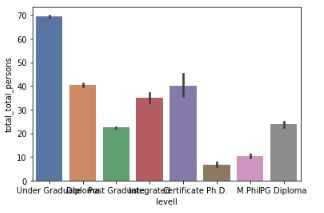
\includegraphics{figures/degrees.jpg}}
\caption{Distribution of students in various degrees}
\label{deg}
\end{figure}

Fig.~\ref{deg} depicts the distribution of the students in different higher education degrees. It is clearly seen that Under graduate degrees are very common and Ph.D degrees are very less in India. This may be due to most Indian students preferring to do their post graduations abroad. 

\begin{figure}[h]
\centerline{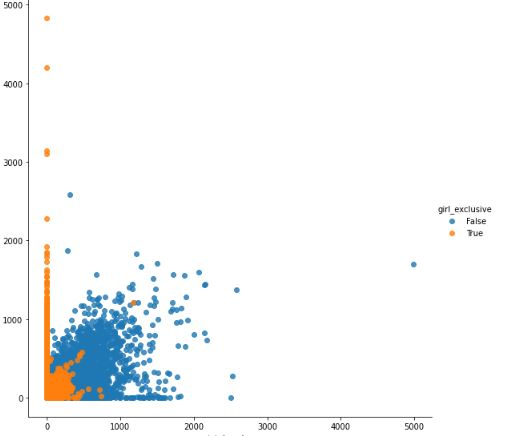
\includegraphics[scale=0.6]{figures/girls_general.jpg}}
\caption{Distribution girls in general category vs muslim girls}
\label{girls}
\end{figure}

In Fig.~\ref{girls}, the number of general community females are plotted against the number of muslim community females and are divided by female exclusive colleges, it is clearly seen that the muslim community prefers to enroll more in female-only colleges as compared to the general category.

Fig.~\ref{study_years} shows the comparison of number of years of study of general caste vs backward castes. A general trend of 1-2 years of study can be seen among backward caste people which shows that they prefer smaller undergraduate degrees and do not often pursue post graduate studies.

\begin{figure}[h]
\centerline{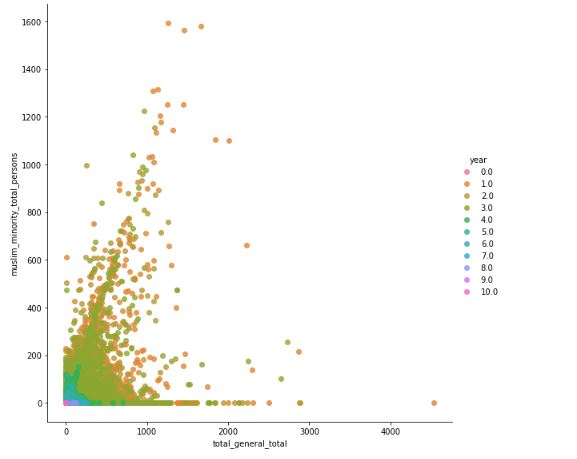
\includegraphics[scale=0.6]{figures/years_study.jpg}}
\caption{Comparison of number of years of study in backward castes vs general caste}
\label{study_years}
\end{figure}

\begin{figure}[h]
\centerline{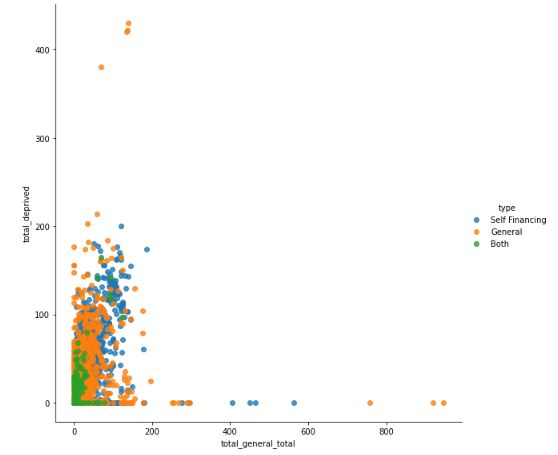
\includegraphics[scale=0.6]{figures/hyd.jpg}}
\caption{Distribution of degrees in Hyderabad based on financial type}
\label{hyd}
\end{figure}

It is observed from Fig.~\ref{hyd} that people in metro cities like Hyderabad prefer self-financing degrees whereas the opposite trend is observed throughout the rest of the country where self-financing is least preferred.

% --------- 6. Mining tasks -----------
\section{Data mining techniques}
After the completion of the pre-processing, three data mining techniques are applied on the dataset. Each mining technique requires presents its own problems and advantages when used on the chosen dataset. The following section gives a comprehensive account of the the three mining techniques applied. 

\subsection{Association rule mining - Apriori}
Association rule mining is chosen as one of the mining techniques to be used on this dataset because the dataset consists of a lot of categorical data. When the categorical data point is viewed as an "item" in the "transaction" (the degree in a particular college, or row), it gives us a means to identify relationships between the the categorical features. 

A significant portion of the pre-processed dataset also consists of ratio data (census data). To fit this information into the association rule mining, the census data is discretized using equal interval binning. The number of intervals and the width of the intervals are chosen by trial and error. The final results are obtained using 4 bins of the following intervals - (0-20), (20-50), (50-70), (70-100). Further, the entire dataset is now converted into a transaction database format to use for association rule mining. 
Apriori rule is chosen as the association rule mining technique as it provides a quick and easy implementation with good results. A major drawback of the apriori rule is that its multiple scans through the dataset takes makes it inefficient for time. But this is not seen as a major drawback in our implementation as the entire process completes in under a minute on the entire dataset.

To get the frequent itemsets and the association rules using the apriori rule, two parameters have to be tuned to get the desired results. These parameters are minimum\_support(or min\_sup) and minimum\_confidence(or min\_conf). By trial and error min\_sup was chosen to be 15\% and min\_conf was chosen to be 60\%. Min\_sup is chosen to be on the lower side because the dataset is highly dimensional and a lot of "items" do not repeat too many times and hence do not form a part of the association rules. To get more interesting rules, the min\_sup was reduced to a lower range of values.

\begin{table}[htbp]
\caption{Association rules using Apriori}
\label{apriori_res}
\begin{center}
\begin{tabular}{|L|L|c|c|}
\hline
 
\textbf{Antecedent} & \textbf{Consequent}& \textbf{Confidence}& \textbf{Lift} \\
\hline
\{PWD[0-20]$^{\mathrm{a}}$, General[20-50], BC[50-70]\} &  \{Co-education\} & 0.894 & 5.251 \\\hline

\{Postgraduate, Co-education\} & \{Muslim[0-20], PWD[0-20], Other[0-20]\} & 0.893 & 4.818 \\\hline

\{Hostel available, No specialty, Undergraduate, Co-education\} & \{PWD[0-20]\} & 0.998 & 4.909 \\\hline

\{No hostel, BC[70-100], PWD[0-20], Other[0-20]\} & \{No specialty\} & 0.881 & 4.696 \\\hline

\{BC[70-100]\} & \{Undergraduate, Co-education\} & 0.682 & 1.791 \\
\hline
% \multicolumn{4}{l}{$^{\mathrm{a}}$The numbers in square brackets represent the percentage of population in that degree in that college}
\end{tabular}
\end{center}
\end{table}

A few results from the Apriori rule are presented in table~\ref{apriori_res}. The numbers in square brackets represent the percentage of population in that degree in that college. BC stands for Backward Castes, PWD for Public Works Department, and Other represents castes other backward castes. 

The first result shows the distribution of the demographic in co-education colleges with 89.4\% confidence. It is observed that PWD are in very low strength as compared to general caste and Backward castes in co-education colleges which may correlate to the less strength of PWD in higher education colleges in general or the more backward thought process of PWD to only take admission in gender exclusive colleges. 
The second result shows that Muslims, PWD and Other backward castes are not likely to enroll in Postgraduate degrees with 89.3\% confidence. This shows that minority groups stop with undergraduate or lower degrees of education. 
The third result confirms the fact that PWD are very less in number even in co-education undergraduate degrees with hostels. No specialty simply means that the degree is not a specialization which is true for all undergraduate degrees. This rule has a very high confidence of 99.8\%.
The last two rules show that Backward castes (BC) are present in high numbers in undergraduate degrees and this is an encouraging sign for a country like India. This could mean that India's reservation system has worked well and now needs to be reformed to focus more on minorities like muslims, PWD, and other backward castes who show a very low representation even in undergraduate degrees.
The results were filtered using scores like confidence and lift and were chosen manually from a final list of 5000+ generated rules.


\subsection{Clustering}

\begin{figure*}[t]
    \centering
    \subfigure[Assigned cluster labels]{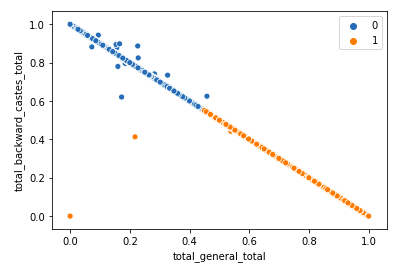
\includegraphics[scale=0.38]{figures/levels1.jpg}}\quad
    \subfigure[Actual labels]{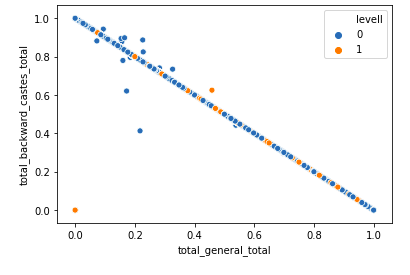
\includegraphics[scale=0.38]{figures/levels2.jpg}}
    \caption{Graphs showing the clustering of different levels of education}
    \label{cluster1_graphs}
\end{figure*}

Given the census-like nature of the dataset, it was decided that clustering could be applied to try and find some interesting results. Upon analyzing the data it is observed that there are 28 numerical attributes, a lot of which are highly sparse, and 10 relevant categorical attributes. 

Cluster analysis can be divided into hierarchical clustering and non-hierarchical clustering techniques. Examples of hierarchical techniques are single linkage, complete linkage, average linkage, median, and Ward. Non-hierarchical techniques include k-means, adaptive k-means, k-medoids, and fuzzy clustering. The goal of K-means clustering is to decrease the summation of square distance among data points and their respective cluster centers. This is an iterative process which eventually converges to output “k” clusters. K-means clustering seemed like the best fit for the dataset because of the census attributes, and the distance between rows would provide information about the differences in population distribution of the rows. Furthermore, some of the categorical attributes have data pertaining to various features like level of education, financing categories for a particular study programme, and exclusivity of females/hostels. These attributes could serve as labels to compare clusters against, after selecting relevant features. In this paper, the traditional K-means clustering algorithm was implemented with Euclidean distance being taken as the distance metric between rows. Reasons for selecting K-means are: simplicity of implementation, speed of convergence and scalability to large datasets such as ours.

Owing to the high dimensionality of the dataset, only a small relevant subset of the numerical attributes are selected for clustering and this relevance is decided by the attribute selected as cluster labels. Upon observing the values for the ``levell'' attribute, it is noticed that the values "Undergraduate" and "Postgraduate" dominated with 326977 and 90643 rows respectively. Thus, k was chosen as two. The attributes "total\_general\_total" and "total\_backward\_castes\_total", the attributes for total general population data and total backward castes data, are chosen for clustering. These attributes are relevant for the aforementioned chosen cluster label attribute, ``levell''. The results obtained are shows in table~\ref{cluster1}. 

At first glance, the precision and recall values look better than expected considering that this was one of the first cluster instances that was performed. However, the plots in Fig~\ref{cluster1_graphs} illustrate the results better. 
It is observed that there is a high precision in the undergraduate sector because it is uniformly spread throughout the dimensions when compared to other degrees and also has a high support count. The high uniformity in the spread is also the reason for the lower recall of the clusters formed here. Whereas, the other degree levels are clustered together near the origin thus when analyzed gives higher recall as all of it can be contained in one cluster but a lower precision as a certain number of undergraduates are also present in the other cluster. Thus clustering does not yield any viable results here.


\begin{table}[htbp]
    \caption{Results of clustering levels of education}
    \label{cluster1}
    \begin{center}
    \begin{tabular}{|c|c|c|c|c|}
    \hline
     
     & \textbf{Precision}& \textbf{Recall}& \textbf{F1 score} & \textbf{Support}  \\
    \hline
    
    label 0$^{\mathrm{a}}$ & 0.79 & 0.69 & 0.74 & 326977 \\\hline
    label 1$^{\mathrm{b}}$ & 0.24 & 0.35 & 0.29 & 90643 \\\hline
    Accuracy &  &  & 0.62 & 417620 \\\hline
    Macro average & 0.52 & 0.52 & 0.51 & 417620 \\\hline
    Weighted average & 0.67 & 0.62 & 0.64 & 417620 \\

    \hline

    \multicolumn{4}{l}{$^{\mathrm{a}}$Undergraduate, $^{\mathrm{b}}$Postgraduate}
    \end{tabular}
    \end{center}
\end{table}

% \begin{figure*}[t]
%     \centering
%     \subfigure[Assigned cluster labels]{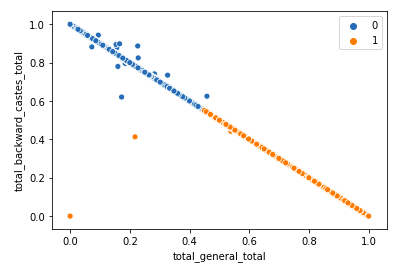
\includegraphics[scale=0.38]{figures/levels1.jpg}}\quad
%     \subfigure[Actual labels]{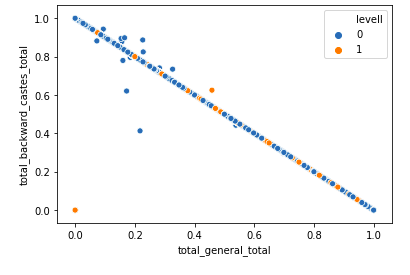
\includegraphics[scale=0.38]{figures/levels2.jpg}}
%     \caption{Graphs showing the clustering of different levels of education}
%     \label{cluster1_graphs}
% \end{figure*}

After considering a few more cluster labels for clustering, like type of college (self financing or not), girl\_exclusive college etc, similar patterns with respect to precision and recall values can be observed, which can be explained by the relevant plots in Fig~\ref{cluster2_graphs}. The results for this clustering are shown in table~\ref{cluster2}.


\begin{figure*}[t]
    \centering
    \subfigure[Assigned cluster labels]{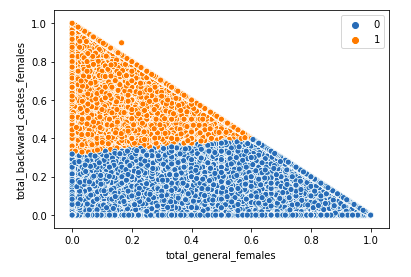
\includegraphics[scale=0.38]{figures/girls2.jpg}}\quad
    \subfigure[Actual labels]{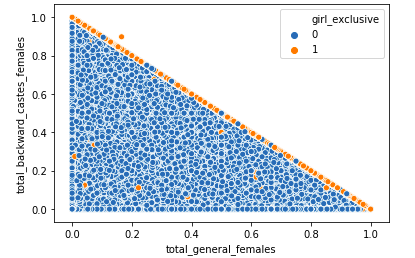
\includegraphics[scale=0.38]{figures/girls1.jpg}}
    \caption{Graphs showing the clustering of gender exclusive colleges}
    \label{cluster2_graphs}
\end{figure*}


\begin{table}[htbp]
    \caption{Results of clustering girls exclusive colleges}
    \label{cluster2}
    \begin{center}
    \begin{tabular}{|c|c|c|c|c|}
    \hline
     
     & \textbf{Precision}& \textbf{Recall}& \textbf{F1 score} & \textbf{Support}  \\
    \hline
    
    label 0$^{\mathrm{a}}$ & 0.93 & 0.75 & 0.83 & 370375 \\\hline
    label 1$^{\mathrm{b}}$ & 0.22 & 0.56 & 0.32 & 47245 \\\hline
    Accuracy &  &  & 0.73 & 417620 \\\hline
    Macro average & 0.58 & 0.66 & 0.58 & 417620 \\\hline
    Weighted average & 0.85 & 0.73 & 0.77 & 417620 \\

    \hline

    \multicolumn{4}{l}{$^{\mathrm{a}}$Not girl exclusive, $^{\mathrm{b}}$Girl exclusive}
    \end{tabular}
    \end{center}
\end{table}

It is thus realized that the cluster label attributes are too skewed towards one of the values for desirable results, and that the available features cannot yield a discernible decision boundary for unsupervised learning techniques such as clustering. 


\subsection{Classification}

The chosen dataset may not seem like a direct fit for a classification task because it is essentially a census dataset. However, classification is attempted on this dataset to find the dependency of all the features of a college degree as a factor in affecting a person's enrollment in that college degree. For example, the task is to find the dependency of features like degree level, number of years of study, location of college, other degree specific features, and also the dependency of the existing demographic of the college on the admission of a minority caste student.

For this classification, the minority caste is chosen to muslims. Hence, the task is to find the dependency of various features on the probability of presence of a muslim in that college degree. There are two output classes which represent if a muslim is likely to be present within that demographic and those types of college degrees. 

The total number of muslims are hence taken as the "Y" and are discretized by using a simple threshold. This threshold is taken as 10\% and depicts that if the population of muslims in a particular college degree are greater than the chosen threshold, it means that they are "present" in that demographic. If their population does not cross this threshold, they are marked as "not present" in that particular college degree.

The required pre-processing techniques were already applied during the general pre-processing step. Features that are relevant for the classification are selected from the pre-processed dataset. The total number of input features are 44. The dataset consists of 375197 examples and these are shuffled and split into train, dev and test sets. Dev and test each consists of 20000 examples and train set contains the rest.

The classification task is carried out using two different learning algorithms - logistic regression and a neural network approach. 

\subsubsection{Logistic regression}
A logistic regression model is trained to predict the presence of a muslim in a particular college degree. Gradient descent is used to optimize the cross entropy loss. L2 regularization is also applied with the regularization parameter $\lambda$ = 10. $\lambda$ is chosen after using a grid search on a logarithmic scale by trying to reduce the variance in the learning (difference between train accuracy and dev accuracy). The accuracies for the logistic regression model are shown in table~\ref{classification_res}.

\begin{table}[htbp]
\caption{Results of classification}
\label{classification_res}   
% \centering
\begin{tabular}{|c|c|c|c|}
\hline
\textbf{} & \textbf{Train accuracy} & \textbf{Dev accuracy} & \textbf{Test accuracy} \\\hline
\textbf{Logistic regression} & 87.42\% & 87.41\% & 87.69\% \\\hline
\textbf{Neural network} & 50.1\% & 12.2\% & 12.4\% \\\hline
\end{tabular} 
\end{table}


\subsubsection{Neural networks}
To try and exceed the performance of the logistic regression model, a neural network is trained to fit the same data. The hyperparameters of the network are chosen by trial and error. Adam is used as the optimizer to optimize the cross entropy loss using a learning rate of 0.0003. The results obtained by training the neural network are far from desirable. The model highly overfits the data as the loss increases with each epoch and the accuracy reduces. Various methods for countering overfitting like regularization at each layer and using dropout layers are implemented but the performance of the model does not increase by a considerable amount. This model is under progress and remains a work that can be implemented in the near future. 

It is observed that logistic regression gives a good enough classifier that can be used to predict whether a student belonging to a certain minority is likely to be present in a given college degree with 87\% accuracy.

% --------- 7. Conclusion -----------
\section{Conclusion}

The Apriori rule gives information about the types of degrees combinations of degrees and college features preferred by different ethnic groups. 
Clustering results in comparison and grouping of different features of the dataset and hence result in the comparison between various ethnic groups by using different factors. Unfortunately, the results of clustering are not satisfactory and do not give rise to good results on this type of a dataset. The failure of clustering algorithms can be attributed to the highly dimensional and varied nature (contains highly dimensional categorical features along with a census data) of the dataset. 
The classification task gives rise to a logistic regression model which can predict the presence of a person from a certain ethnic group in a college degree based on the features of the degree and also the existing ethnic groups in the college degree. The neural network approach did not yield good results but can be a promising project in the near future.
To conclude, the three data mining techniques applied give us different valuable insights into the patterns in higher education enrollment in the country. These results can be used for a better analysis and understanding of the education trends of different ethnic groups and genders in India. Moreover, this paper deals with the analysis of and implementation of 3 data mining techniques on a large, sparse, high dimensional, categorical, and census data, and hence serves as a guide for applying basic data mining tasks on such datasets.

% --------- References -------s
\begin{thebibliography}{00}

\bibitem{b1} "Student Enrollment for Regular Courses of Colleges, 2015-16", Data.gov.in, 2020. [Online]. Available: https://data.gov.in/resources/student-enrollment-regular-courses-colleges-2015-16.

\bibitem{b2} Agrawal, Rakesh, and Ramakrishnan Srikant. ”Fast algorithms for mining association rules.” In Proc. 20th int. conf. very large data bases, VLDB, vol. 1215, pp. 487-499. 1994.

\bibitem{b3} Nadig, "Implementing K Means Clustering from Scratch - in Python", The Nadig Blog, 2020. [Online]. Available: http://madhugnadig.com/articles/machine-learning/2017/03/04/implementing-k-means-clustering-from-scratch-in-python.html.

\bibitem{b4} https://github.com/Ravi-0809/data\_mining

\bibitem{b5} "Basic Information of Colleges, 2015-16", Data.gov.in, 2020. [Online]. Available: https://data.gov.in/resources/basic-information-colleges-2015-16.

\end{thebibliography}


\end{document}
